
\chapter{Dynamic Component Model}

This chapter covers the architecture of the dynamic component model of U-Sem which enables scientists to dynamically load and use custom functionality.


\section{Problem definition}

All of initial interviews with potential users of the system reviled that the nature of their work is extremely dynamic. The main responsibility of the scientists is to come up with new algorithms and approaches for user modelling. As a result they are continuously producing new software code that implements this algorithms. After each production cycle, this program code has to be put into U-Sem so that it is  available for testing, demonstration and evaluation purposes.

We performed additional interviews with stakeholders in order to reveal how this process is currently done. Scientists reported that they have on their disposal only the capabilities of the workflow engine. However, it provides no functionality that enables to plug custom logic on demand into the system and as a result scientists are forced to "hardcode" their logic into the source code of the workflow engine. In this way the software code implementing the algorithms become part of the workflow engine. This approach is error prone and brings a lot of discomfort to the scientists working with the system. The most important disadvantages of this approach include:

\begin{itemize}

	\item Adding new functionality requires a lot of time and knowledge. This is because in order to add the new functionality one has to alter the source code of the workflow engine and basically release a new version of it. This process requires advanced knowledge about each phase of the process: checking out the source code from the software repository, writing the new source code in the appropriate place, building the system and finally deploying it to the web server. Most of the time, all this knowledge is not required for the daily work of scientists and learning it creates a serious overhead and discomfort.
	
	\item In order to add new functionality to the system one has to stop the web server where the system is deployed, replace the program entities of the system and start the server again. The problem is that during the time the server is down all previously created services are unavailable. This is a major problem for everyone that is using the system during that time.
	
	\item Another major disadvantage is that the training period for new scientist working with the system is significant because of all the additional knowledge required. This may easily cause project delays and missed deadlines.
	
	\item Multiple scientists adding functionality simultaneously result in missing functionality. \textbf{Figure 1} illustrates the problematic scenario. As stated earlier in order to add new functionality scientists must first check out the source code of the system, make the changes and deploy the new version on the web server. However, if two scientist perform this process simultaneously then the new functionality provided by the first scientists will be lost when the second deploys his version. 
	
	\item It is hard to verify what additional functionality is added to the system and therefore, additional documentation is required. This problem becomes more serious when there are more people are working on the project simultaneously and it is hard to track the changes in functionality.
		
\end{itemize}

But this is not everything. This approach also introduces one big disadvantage from software engineering perspective. The problem lies in the poor modularization of the system. In software engineering modularization is considered a key property for improving extensibility, comprehensibility, and reusability in software projects \cite{Parnas}. In this case, engineers can only rely on the modular functionality provided by the Java language. However, its information hiding principles are only applied on class level, but not to the level of packages and JAR files. For example, it is not possible to restrict access to certain public classes defined in a package. The absence of such visibility control can easily lead to highly coupled,"spaghetti-like" systems. The consequences of this will become more and more clear with the time when the system grows in size, complexity and the number of engineers working on it increases. The most probable consequences include high development costs, low productivity, unmanageable software quality and high risk to move to new technology \textbf{Cai}.

When designing the U-Sem architecture we considered all these pitfalls of the current approach. However, before going to the architecture description, for clarity and easier validation, in the next subsection, we provide a more formal representation of all user requirements.


\subsection{Functional Scenarios}
In this section we are formally identify the functional requirements which define the main interactions between the scientists and the system. This compact representation of the requirements also makes validation an evaluation clearer. 

\begin{itemize}

	\item \textbf{Creating custom functionality} - This is the main scenario regarding the dynamic component model. Scientists has to be able to extend U-Sem by adding custom functionality on demand. They has to be able to be able to compose the custom functionality independently from the system, add the produced functionality to U-Sem during the execution time of the system and/or if desired share it with other scientists.
	
	\item \textbf{Use functionality shared by other scientists} - Scientists has to be able to reuse custom functionality provided by other scientist.
	
	\item \textbf{Manage loaded functionality} - Users has to able to manage all functionality already added to the system. This includes to be able to view a list of all added functionality. And secondly they have to be able to remove any functionality from the provided list.
			
	
\end{itemize}

\subsection{Non-functional requirements}

This section defines the main quality scenarios of the system that model how the system should react to a change in its environment.

\begin{itemize}

	\item Availability - adding custom functionality should not affect other users at all.
	
	\item Insulation - scientists not being affected by any future changes to the reused components.
	
	\item Privacy - As a user, I don't want other users to see what is my custom functionality and use them.
	
	\item Security
	
\end{itemize}

\section{Approach}

After a detailed investigation of the requirements we reached the conclusion that the core of the problem lies firstly in the poor separations of concerns(modularization) and secondly the impossibility to manage(add, replace, remove) these concerns while the system is in operation. In order to solve these problems we investigated the scientific literature to find what are the available approaches and technologies that help to overcome these problems. The review showed that the topic about modularization of software systems is widely discussed and there is even a sub field in software engineering which addresses the problem of building a system out of different components \cite{Jifeng}. It is called Component-based software engineering. 

Next subsection discusses the basic idea and advantages that this approach brings. Then we discus what features a system needs to provide in order to enable Component-based software engineering. This is known as component model. At the end we also discuss the state of the art technologies that provide support for Component-based software engineering, enable dynamic management of the components and are useful in the context of U-Sem. 

\subsection{Component-based software engineering}

Component-based software engineering is based on the idea to construct software systems by selecting appropriate off-the-shelf components and then to assemble them together with a well-defined software architecture \cite{Pour}. This software development approach improves on the traditional approach since applications no longer has to be implemented from scratch. Each component can be developed by different developers using different IDEs, languages and different platforms. This can be shown in \textbf{Figure 1}, where components can be checked out from a component repository, and assembled into the desired software system.

\begin{figure}[h!]
  \centering
  	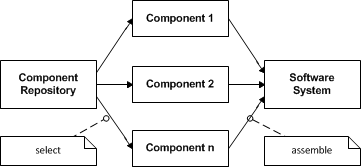
\includegraphics[scale=0.75]{plug-in/component-based.png}
  \caption{Component-based software development \textbf{cite 335} }
\end{figure}

The main benefits that Component-based software development brings are: significant reduction of development cost and time-to-market, and also improvement on maintainability, reliability and overall qualities of software systems \cite{Pour1} \cite{Pour2}. Additionally, the applicability of this this approach is supported by the fact that is widely used in both the research community and in the software industry. There are many examples of technologies implementing this approach including: OMG's CORBA,  Microsoft's Component Object Model(COM) and Distributed COM (DCOM), Sun's(now Oracle) JavaBeans and Enterprise JavaBeans, OSGI.

\subsection{Component model}

A component model is the architecture of a system or part of a system that is built using components \cite{Cai}. It defines a set of  standards for component implementation, documentation and deployment. Usually, the main components that a component-based software system consists of are \cite{Chen}:

\paragraph{Interfaces}
	determine the external behaviour and features of the components and allow the components to be used as a black box. They provide the contract which defines the means of communication between components. As illustrated on \textbf{fig} interfaces can be considered as points where custom functionality provided by another component can be plugged in. 
	
	\begin{figure}[h!]
  		\centering
  		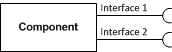
\includegraphics[scale=0.75]{plug-in/component-interfaces.png}
  		\caption{Component interfaces }
	\end{figure}

\paragraph{Components}
	are functional units providing functionality by implementing interfaces. As you can see on \textbf{figure} components provide  features by implementing the provided interface. One of the main question regarding building components is how to define the scope and characteristics for a component. According to \cite{Cai} there are no clear and well established standards or guidelines that define this. In general, however, a component has three main features: 

\begin{itemize}
	\item a component is an independent and replaceable part of a system that fulfils a clear function
	\item a component works in the context of a well-defined architecture
	\item a component communicates with other components by its interfaces 
\end{itemize}

	\begin{figure}[h!]
  		\centering
  		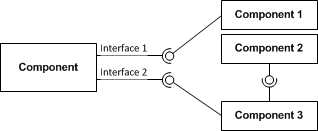
\includegraphics[scale=0.75]{plug-in/component-services.png}
  		\caption{Components implementing interfaces }
	\end{figure}

\paragraph{Coordinator}
	is the entity which is responsible to glue together and manage all the components. It is needed because components provide a number of features, but they are not able to activate the functionality themselves. This is the responsibility of the coordinator.

\subsection{State of the art component model implementations}

Previous sections clearly show that integrating component model in the architecture of U-Sem will solve the design problem of will fulfil the requirements of the customers. Nowadays, there are many implementation of component models and it might be wiser to reuse one of them instead of implementing everything from scratch. The reasons for doing that are because this implementations are developed for long time, they are popular and widely used. This suggests that they are heavily tested and thus provide higher quality. 

\cite{Lau} suggests classification of the component model implementations based on which part of the life cycle of a system the composition of the components is done. They identify the following groups:

\begin{itemize}
	\item  Composition happens during the design phase of the system. Components are designed and implemented in the source code of the system.
	\item  Composition happens during the deployment phase. Components are constructed separately and are deployed together into the target execution environment in order to form the system.
	\item Composition happens during the runtime phase. Components are put together and executed in the running system.
\end{itemize}

For the architecture of U-Sem we are only interested in the last group since one of the main requirements is that scientists should be able to add, update and remove components while the system is running without restarting it. It is essential since the system is used by multiple scientists and any system restart will cause temporary unavailability of all services. 

Apart form this, there is also another critical concern when choosing component model implementation for U-Sem. The implementation should support the Java language since it is the language in which all current services are implemented and also having to learn a new language is considered as a big disadvantage for the scientists.

We performed an investigation in order to find what are the current state of the art technologies that satisfy all requirements. It showed that currently there two standards that satisfy our needs: Fractal \cite{Bruneton} and Open Services Gateway initiative (OSGI) \cite{OSGI}. For U-Sem we chose to use OSGI since our impression is that it provides a simpler way of defining components(no component hierarchies) which will be beneficial for scientists that do not have so in depth knowledge of component-based engineering. OSGI is also widely used\cite{Andre} which may suggest that it is extensively tested and therefore is more stable. Next subsection focuses on how OSGI works and its features that are interesting for the architecture of U-Sem.


\subsection{OSGI}

Proposed first in 1998, OSGI represents is a set of specifications that implement the component model and defines a dynamic component system for Java. These specifications enable a development model where applications are dynamically composed of different independent components. Components can be loaded, updated and deleted on demand without having to restart the system. OSGI implements the main components of the standard component model which are discussed in the previous section as follows:

\begin{figure}[h!]
  \centering
  	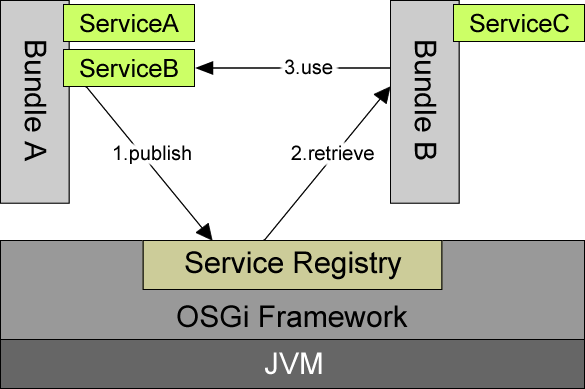
\includegraphics[scale=0.6]{plug-in/OSGI.png}
  \caption{OSGi Service Registry \cite{Andre}}
\end{figure}

\paragraph{Interfaces}
 in OSGI define the contract for communication between different components by describing the operations that has to be implemented by the components. Basically, they represent standard Java interfaces which has to be available to both the component that implements the interface and the components that use the implemented functionality.


\paragraph{Components}
  in OSGI are called bundles. Bundles are basically a regular Java JAR files that contain class files and other resources such as images, icons, required libraries. OSGI also provides facilities for better information hiding then the one provided by the Java language \cite{Andre}. Each bundle should provide a manifest file, which enables engineers to declare static information about the packages that are exported and therefore can be used by other bundles. Furthermore, bundles provide functionality to the rest of the system in the form of services. In the OSGi architecture, services are standard Java objects that implement the required  Interfaces explained in the previous paragraph.

\paragraph{Coordinator}
The OSGi standard also provides coordinator component which represents a runtime infrastructure for controlling the life cycle of the bundles which includes adding, removing and replacing bundles at run-time, while preserving the relations and dependencies among them. Another key functionality that the coordinator component of OSGi provides is the management of the services provided by the bundles. This is provided by the Service Registry, which keeps track of the services registered within the framework. As illustrated in \textbf{Figure 1} when a bundle is loaded it registers all the services that it implements(step 1). As soon as it is registered it can be retrieved by any other components that are interested in this functionality (step 2). Once a bundle has retrieved a service, it can invoke any method described by the interface of this service (step 3). Another interesting feature of the OSGi Service Registry is its dynamic nature. As soon as a one bundle publishes a service that another bundle is interested in, the registry will bind these two bundles. This feature is very important for U-Sem since it will enable scientists to plug in any new functionality dynamically when it is needed.


\section{Architecture}



\subsection{Runtime environment}

This section discusses the runtime environment of U-Sem. As explained in the introduction section initially the system only communicated with providers of semantic content and the clients which execute the services. However, introducing the dynamic component model of U-Sem we bring to entities on the stage. \textbf{Figure} illustrates the updated runtime environment of U-Sem.

\paragraph{Scientists}
As one can see on the diagram the system also communicates with the scientists in order to enable them to plug-in new functionality. When scientists want to add new functionality they first have to build a component that encapsulates the new logic. Then they upload the component to U-Sem and it will be installed in the components space of the scientist. Once installed, the scientist can start using the newly added functionality. Scientists can also communicate with U-Sem in order to manage the existing components loaded into the system. They can view the list of all available components and if needed they can also update or even remove them. 

\begin{figure}[h!]
  \centering
  	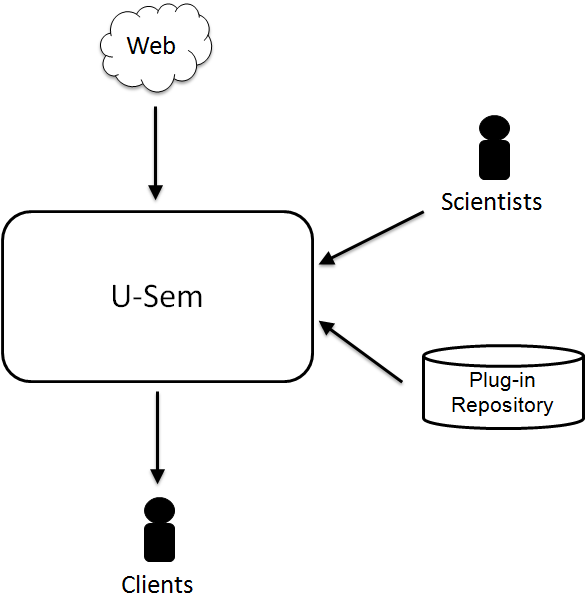
\includegraphics[scale=0.5]{plug-in/environment/runtime_env.png}
  \caption{Runtime environment in U-Sem }
\end{figure}

\paragraph{Plug-in repository}
Another interesting addition to the environment is the Plug-in repository. It represents a storage location where plug-ins are stored and when needed, they can be retrieved and installed into the system. Scientists build and then publish their plug-ins there so that anyone interested can install and use them. The need for this approach emerges from the fact that scientists has to be able to share their components with one another.

By using the Plug-in repository scientists are able to share components before they are installed into U-Sem. Alternative approach would have been enable scientists to share already installed components between each other. In this way whenever a scientist creates a new version or entirely new component it is installed to U-Sem, shared and then all other scientists are able to use it. However, this approach has one major disadvantage. When a new version of a component is installed then all scientists automatically start to use the new version. The version, though, might introduce a bug or it might not be completely compatible with the previous version. As a result, all other scientists' services and components that are using it are threatened to experience failures. 

Using the Plug-in repository overcomes this problem. When a scientist releases new version of component, other scientists can decide whether or not to immediately adopt the new release. If they decide not to, they can simply continue using the old one. Otherwise, when they decide that are ready for the change, they install and use the new release. The benefit from this is that none of the scientists are at the mercy of the others. Changes made to one component do not need to have an immediate affect on other scientists that are using it. Each scientist can decide weather or when to move to the new releases of the components in use. This approach is already adopted in the industry \textbf{TODO P2, Eclipse etc.}


\subsection{Process modelling}

Once we have already identified the new actors(scientists) and external systems(plug-in repository) in the runtime environment of U-Sem we have to define how they interact between each other. In this section we will use the Business Process Management Notation(BPMN) \cite{BPMN} to model the business processes that defines the interactions needed in each of the use cases that regard the dynamic component model feature of U-Sem. It also enables to model activities, decision responsibilities, control and data flows. The decision to use BPMN to model the interactions is based on its relative suitability for interaction modelling and the fact that it is more popular compared to its alternatives \cite{Decker}. Next subsections describe each of the defined processes and expand them into Business Process Diagrams (BPD).

\subsubsection{Create U-Sem Component process}

Creating new functionality for U-Sem is the most important use case regarding the dynamic component model feature. We modelled this use case as the \textit{Loading new components} business process. \textbf{Figure} provides the business process model diagram that illustrates this process. 

As illustrated in the diagram there are three participants in this process(U-Sem, Scientists and Plug-in repository) which are illustrated in separate BPMN pools. When a scientist wants to create new functionality for U-Sem, he/she firsts writes the source code, providing all required resources and implementing the desired U-Sem interfaces(the component interfaces discussed in previous sections). Then everything has to be build and encapsulated into a component. Once the component is ready, scientists can directly upload it to U-Sem if the component is only for private use. When U-Sem receives a component it is responsible to installed it into the scientist's component storage please and make available all functionality provided by the component. Finally, U-Sem sends confirmation message back to the scientist. Alternatively the scientist might also want to share the component with other scientists. In this case the component is sent to the plug-in repository. When received, the repository is responsible to store it and make it available to the other scientists. Again at the end confirmation message is send to the scientist.

\begin{figure}[h!]
  \centering
  	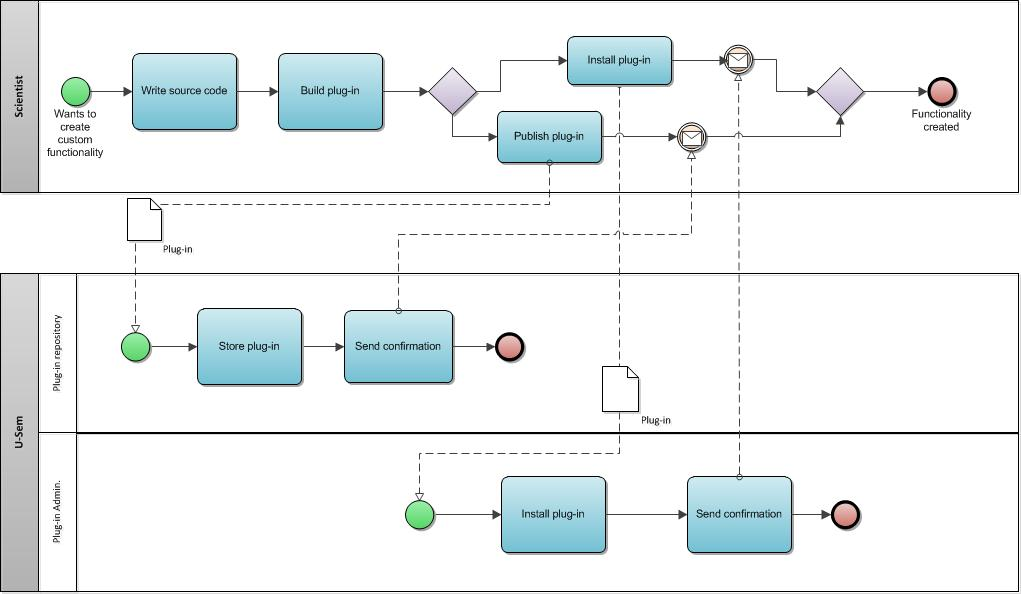
\includegraphics[scale=0.7,angle=90]{plug-in/business_processes/CreatePlugInBusinessModel.jpg}
  \caption{Business model describing the process for adding new plug-in to U-Sem}
\end{figure}

\subsubsection{Reuse shared components}

As already explained, U-Sem also enables scientists to reuse components shared by other scientist. This use case is modelled into the \textit{Reuse shared components} business process which is illustrated in \textbf{figure}. Again we have three participants in this process(U-Sem, Scientists and Plug-in repository) which are illustrated in separate BPMN pools. 

The process consists of two main phases. First, the scientist contacts the plug-in repository in order to determine what are the currently available components. Secondly, he/she contacts U-Sem providing information about the desired component/s. U-Sem then contacts the plug-in repository in order to get the components. Finally, the provided components are stored into the private space of the scientist and a confirmation message is send back.

\begin{figure}[h!]
  \centering
  	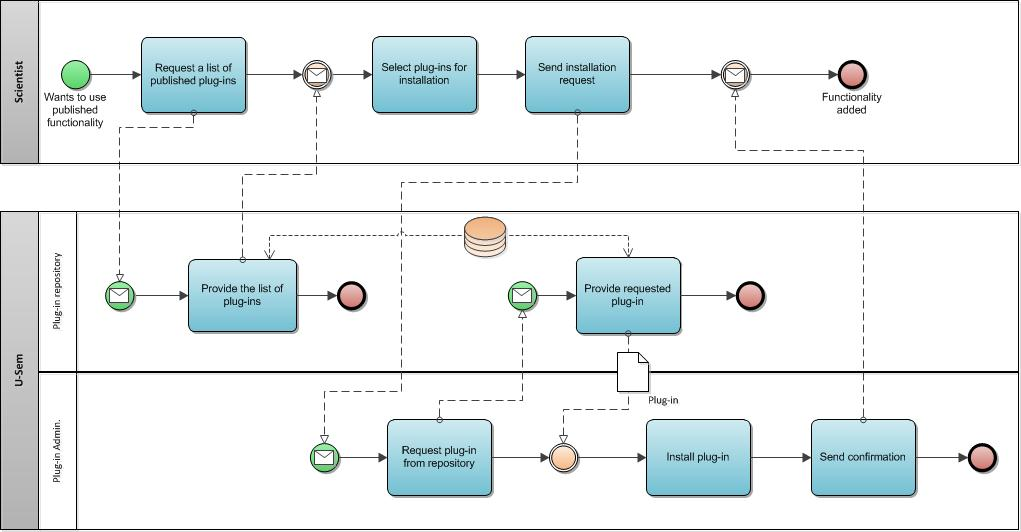
\includegraphics[scale=0.7,angle=90]{plug-in/business_processes/InstallPlugInFromRepoBusinessModel.jpg}
  \caption{Business model describing the process for adding existing plug-in from repository to U-Sem}
\end{figure}

\subsubsection{Component Management}

Managing components is also another important use case. Implementing it will enable scientists to view all components installed into U-Sem and if needed remove them. This use case was modelled into the \textit{Component Management process} which is illustrated on \textbf{Fugure}. In this case we have interaction only between the scientist and U-Sem.

Scientists can monitor the currently installed components at any time by contacting U-Sem. When such request is received, U-Sem is responsible to send back detailed information about all the components. Having this lists, scientist are also able to remove components. In this case scientists have to submit request for removal providing detailed for the component that has to be removed. Upon receiving such request U-Sem is responsible to permanently remove the component form the private space of the scientists and when finished send back a confirmation message.

\begin{figure}[h!]
  \centering
  	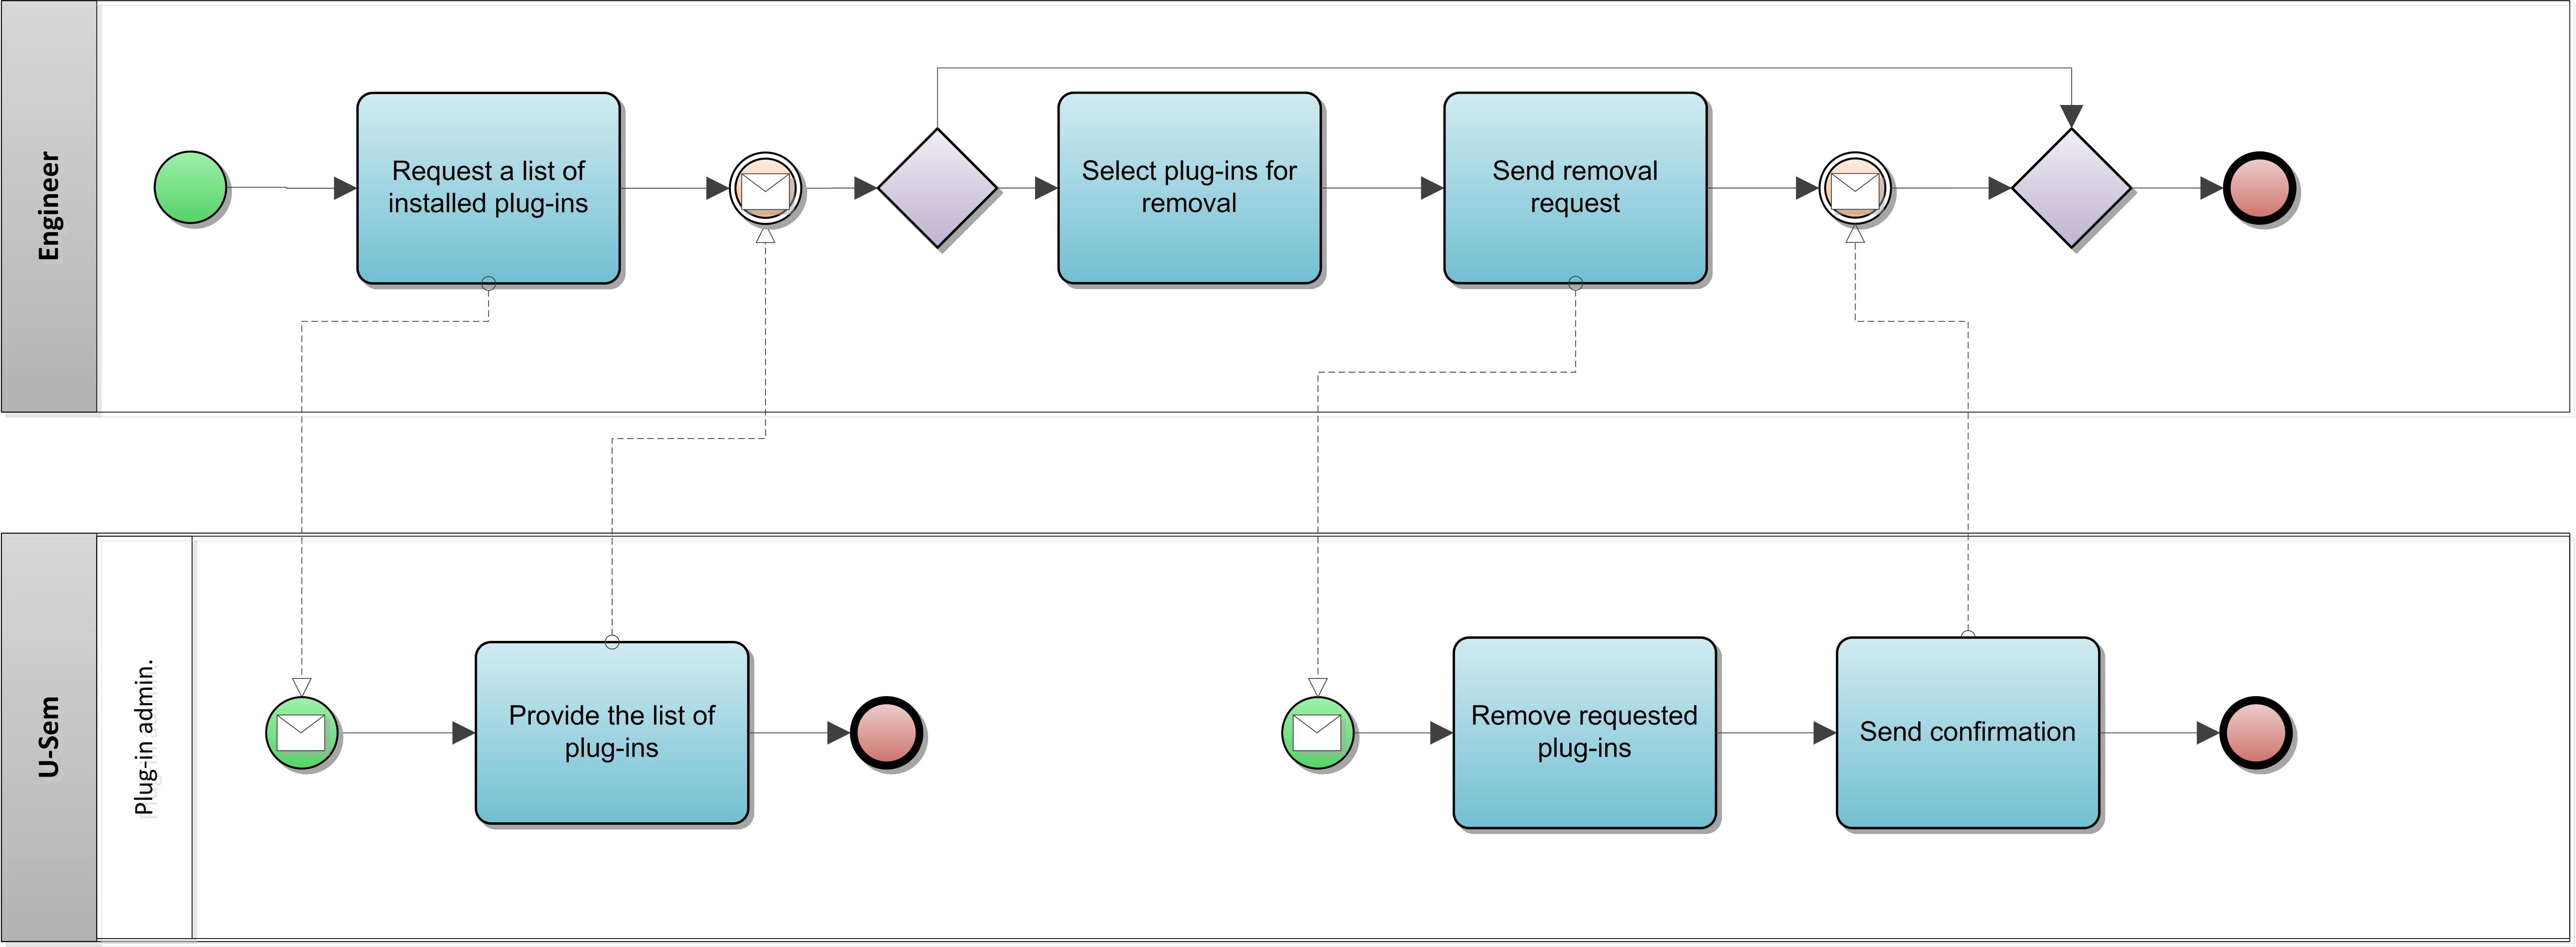
\includegraphics[scale=0.6]{plug-in/business_processes/PluginManagementBusinessModel.jpg}
  \caption{Business model describing the process for managing plug-ins in U-Sem}
\end{figure}


\subsection{Functional organization}

After identifying all actors that that are part of the environment of U-Sem and the way they interact with one another, it is now time to discuss the internal structure of U-Sem that accommodates all these interactions. This section defines the architectural elements that provide the functionality of the system. It describes the functional structure of the system including the key functional elements, their responsibilities, the interfaces they expose, and the interactions between them. Taken together, this demonstrates how the system will perform the required functions.

All components that are take part in the dynamic component model functionality can be classified in layers. This three layered organization is illustrated in figure \textbf{Figure} and defines the following layers:

\begin{figure}[h!]
  \centering
  	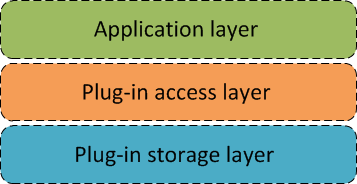
\includegraphics[scale=0.6]{plug-in/layers/layers.png}
  \caption{Layer organization of U-Sem}
\end{figure}

\begin{itemize}
	\item \textit{Plug-in storage layer} is responsible to provide storage functionality for plug-ins.
	\item \textit{Plug-in access layer} provides functionality for plug-in management and provides access to services provided by the components. Components in this layer are responsible to enforce the security, privacy, etc. policies of the system.
	\item \textit{Application layer} this layer consists of all components that are interested in using the services provided by the plug-ins. These applications are also responsible to provide functionality to the user for adding new plug-ins to the system or managing the existing once. 
	\end{itemize}

\subsubsection{High-level organization}

This section describes the internal structure of the layers and specifies the high level components that build up the feature. \textbf{Figure} illustrates this organization and shows how the components are organized into the layers. We have the following components starting from bottom up:\textbf{TODO better explanation is needed}

\begin{figure}[h!]
  \centering
  	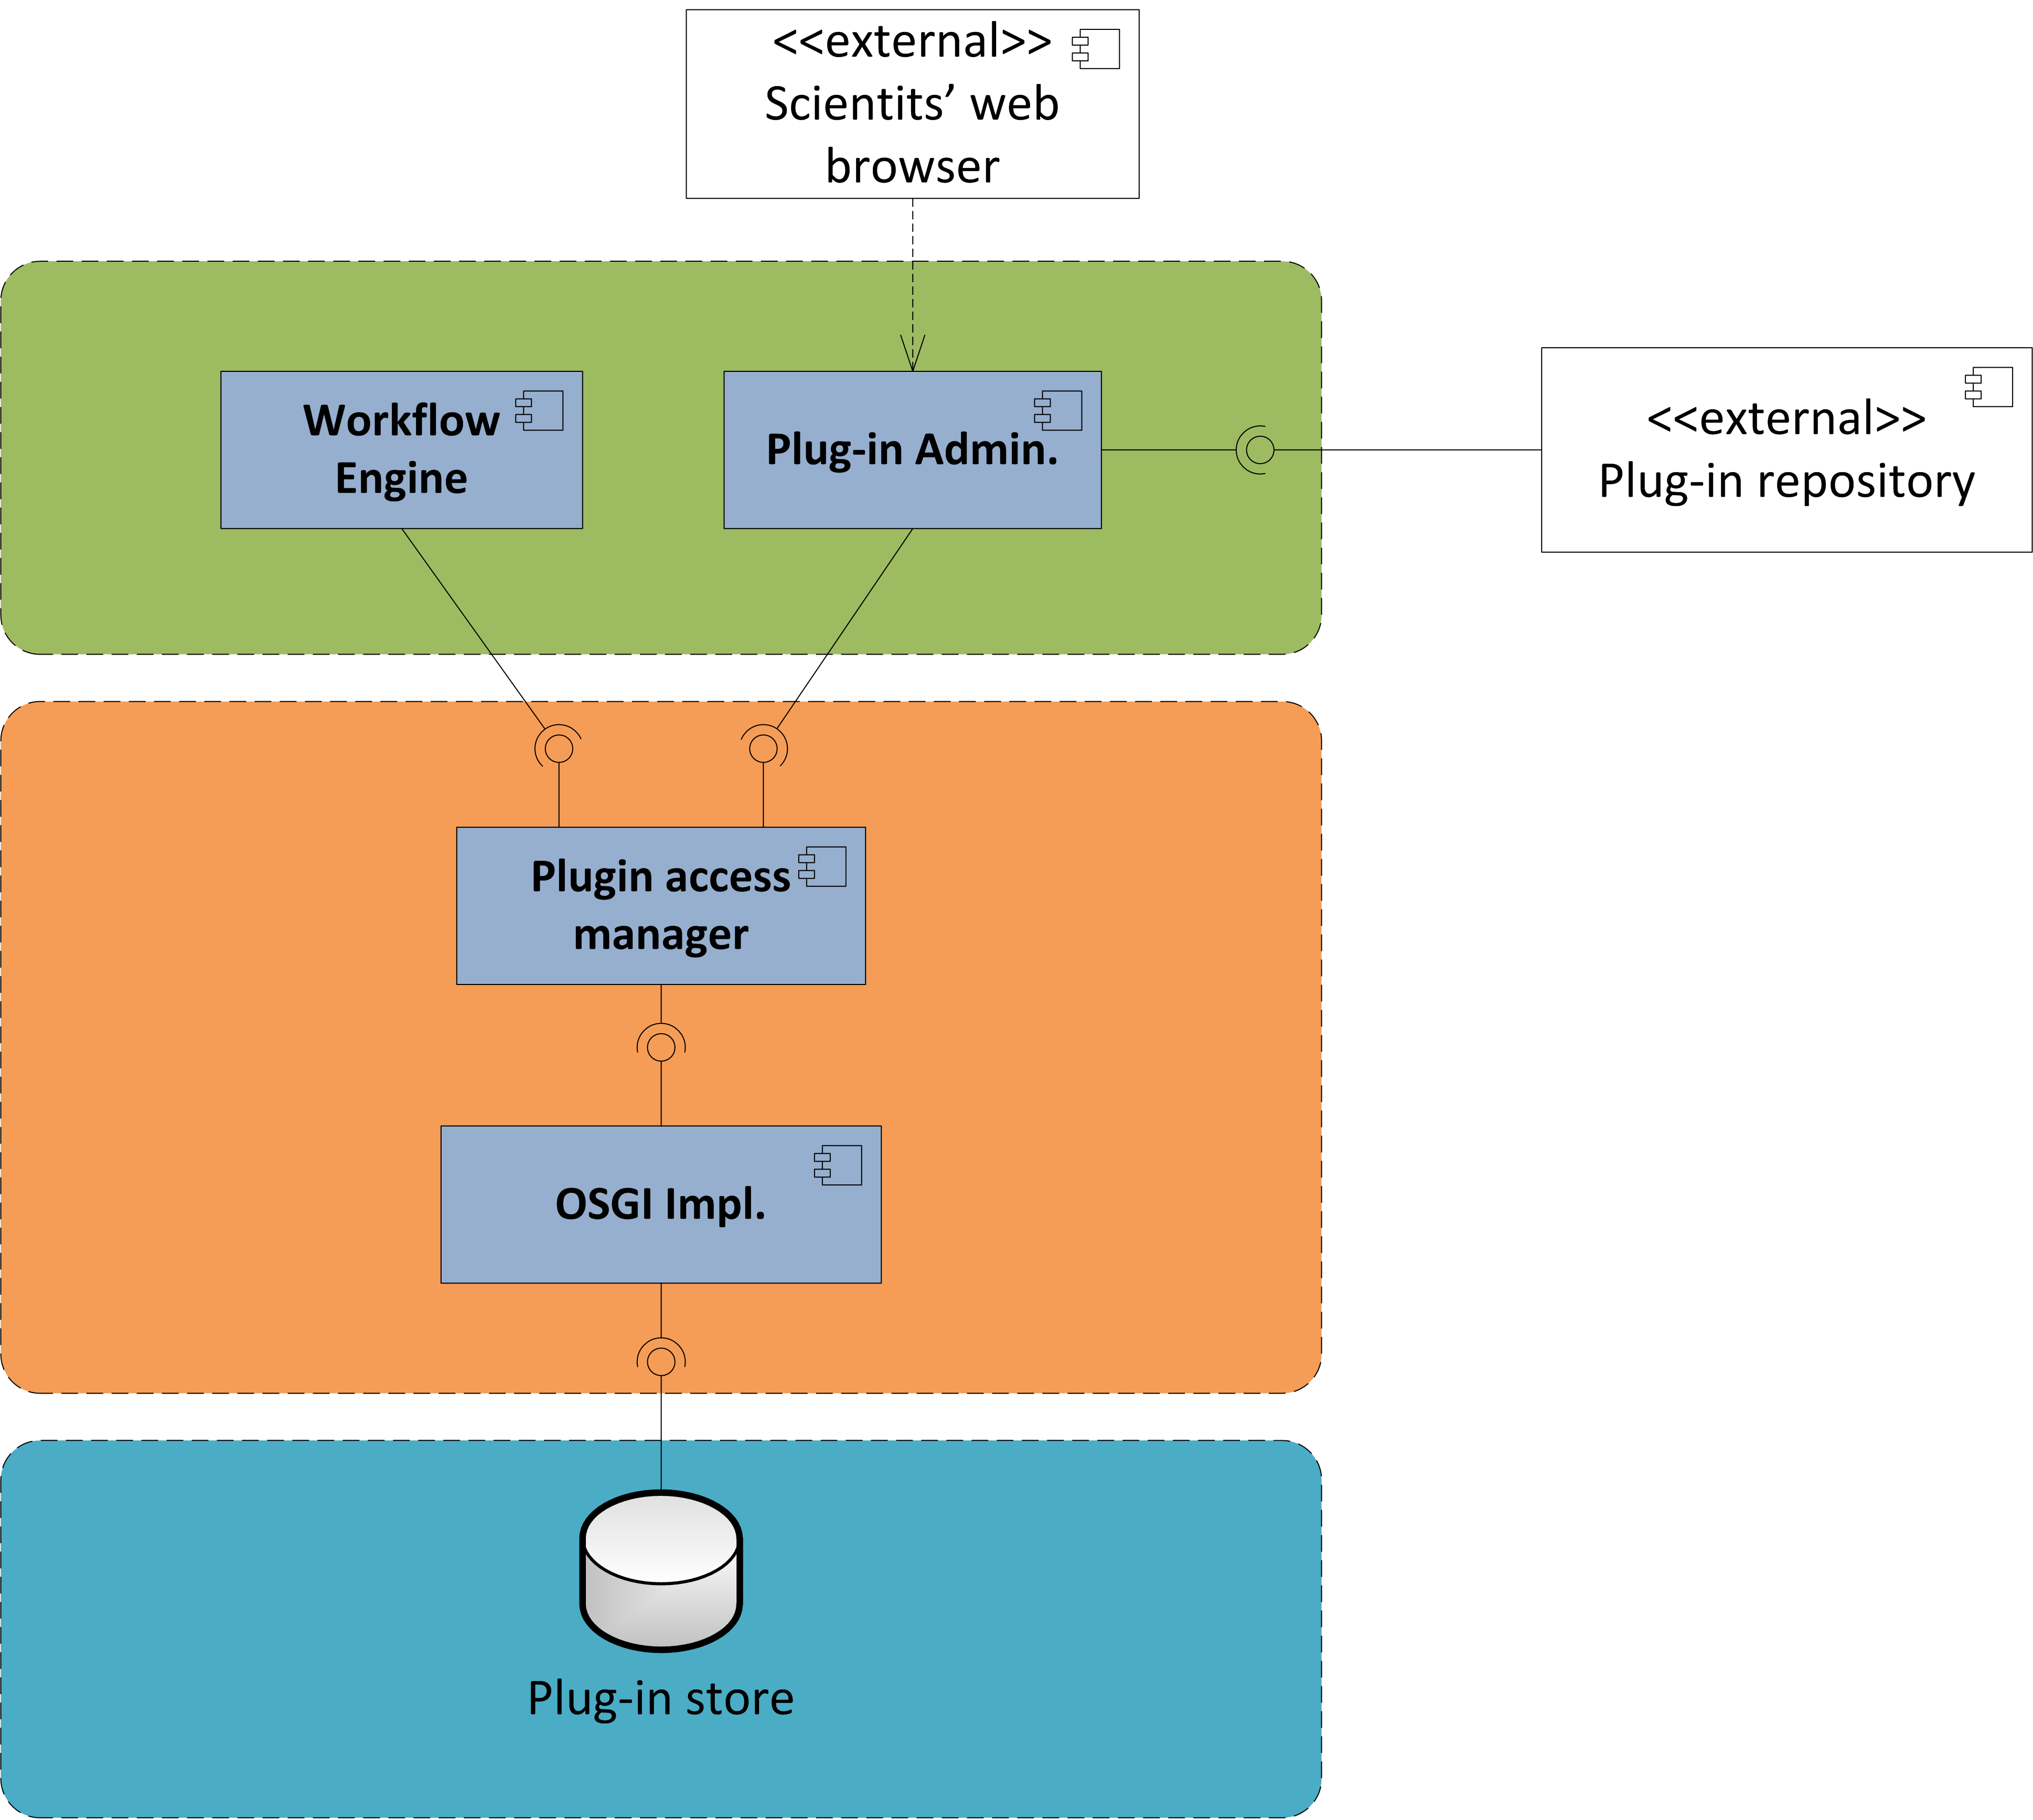
\includegraphics[scale=0.6]{plug-in/layers/main-func.png}
  \caption{Layer organization of U-Sem}
\end{figure}

\begin{itemize}

\item \textit{Plug-in Store} is responsible to store the installed plug-ins for each user. It should provide permanent store for the components so that after system restart they are still available. This component is also responsible to provide storage space for each component in case any data storage is required. Current implementation of OSGI can only operate with file store and therefore this component is represented by the file system of the operating system. For availability reasons this storage should be \textbf{replicated}.

\item \textit{OSGI Implementation} - As we already discussed in previous sections, we chose OSGI as a standard for achieving the dynamic component model for U-Sem. It is responsible to keep track of plug-ins life cycle(create, store, ..) and provide access to the services implemented by the different components. It provides API which enables communication with the framework.

\item \textit{Plug-in access manager} acts as a level of abstraction over the OSGI component. It is responsible to deal with the configuration ans start of the framework. It is also responsible to enforce the security policy and provide insulation between scientists. It provides API for the higher level components for dealing with services and management of plug-ins. Further decomposition of this component is provided in the next section.

\item \textit{Plug-in admin.} is responsible to deal with the administration of the plug-ins. It provides the system's endpoint(UI) for interaction with the scientist scientists. Further decomposition of this component is provided in the next section. 

\item \textit{Workflow engine} uses the interface provided by the \textit{Plugin access manager} to get list of the available services and when required execute them.
	
\end{itemize}


\subsubsection{Plug-in admin. module}

\textbf{Figure} shows the functional decomposition of the Plug-in admin. module. It consists of the following components:

\begin{figure}[h!]
  \centering
  	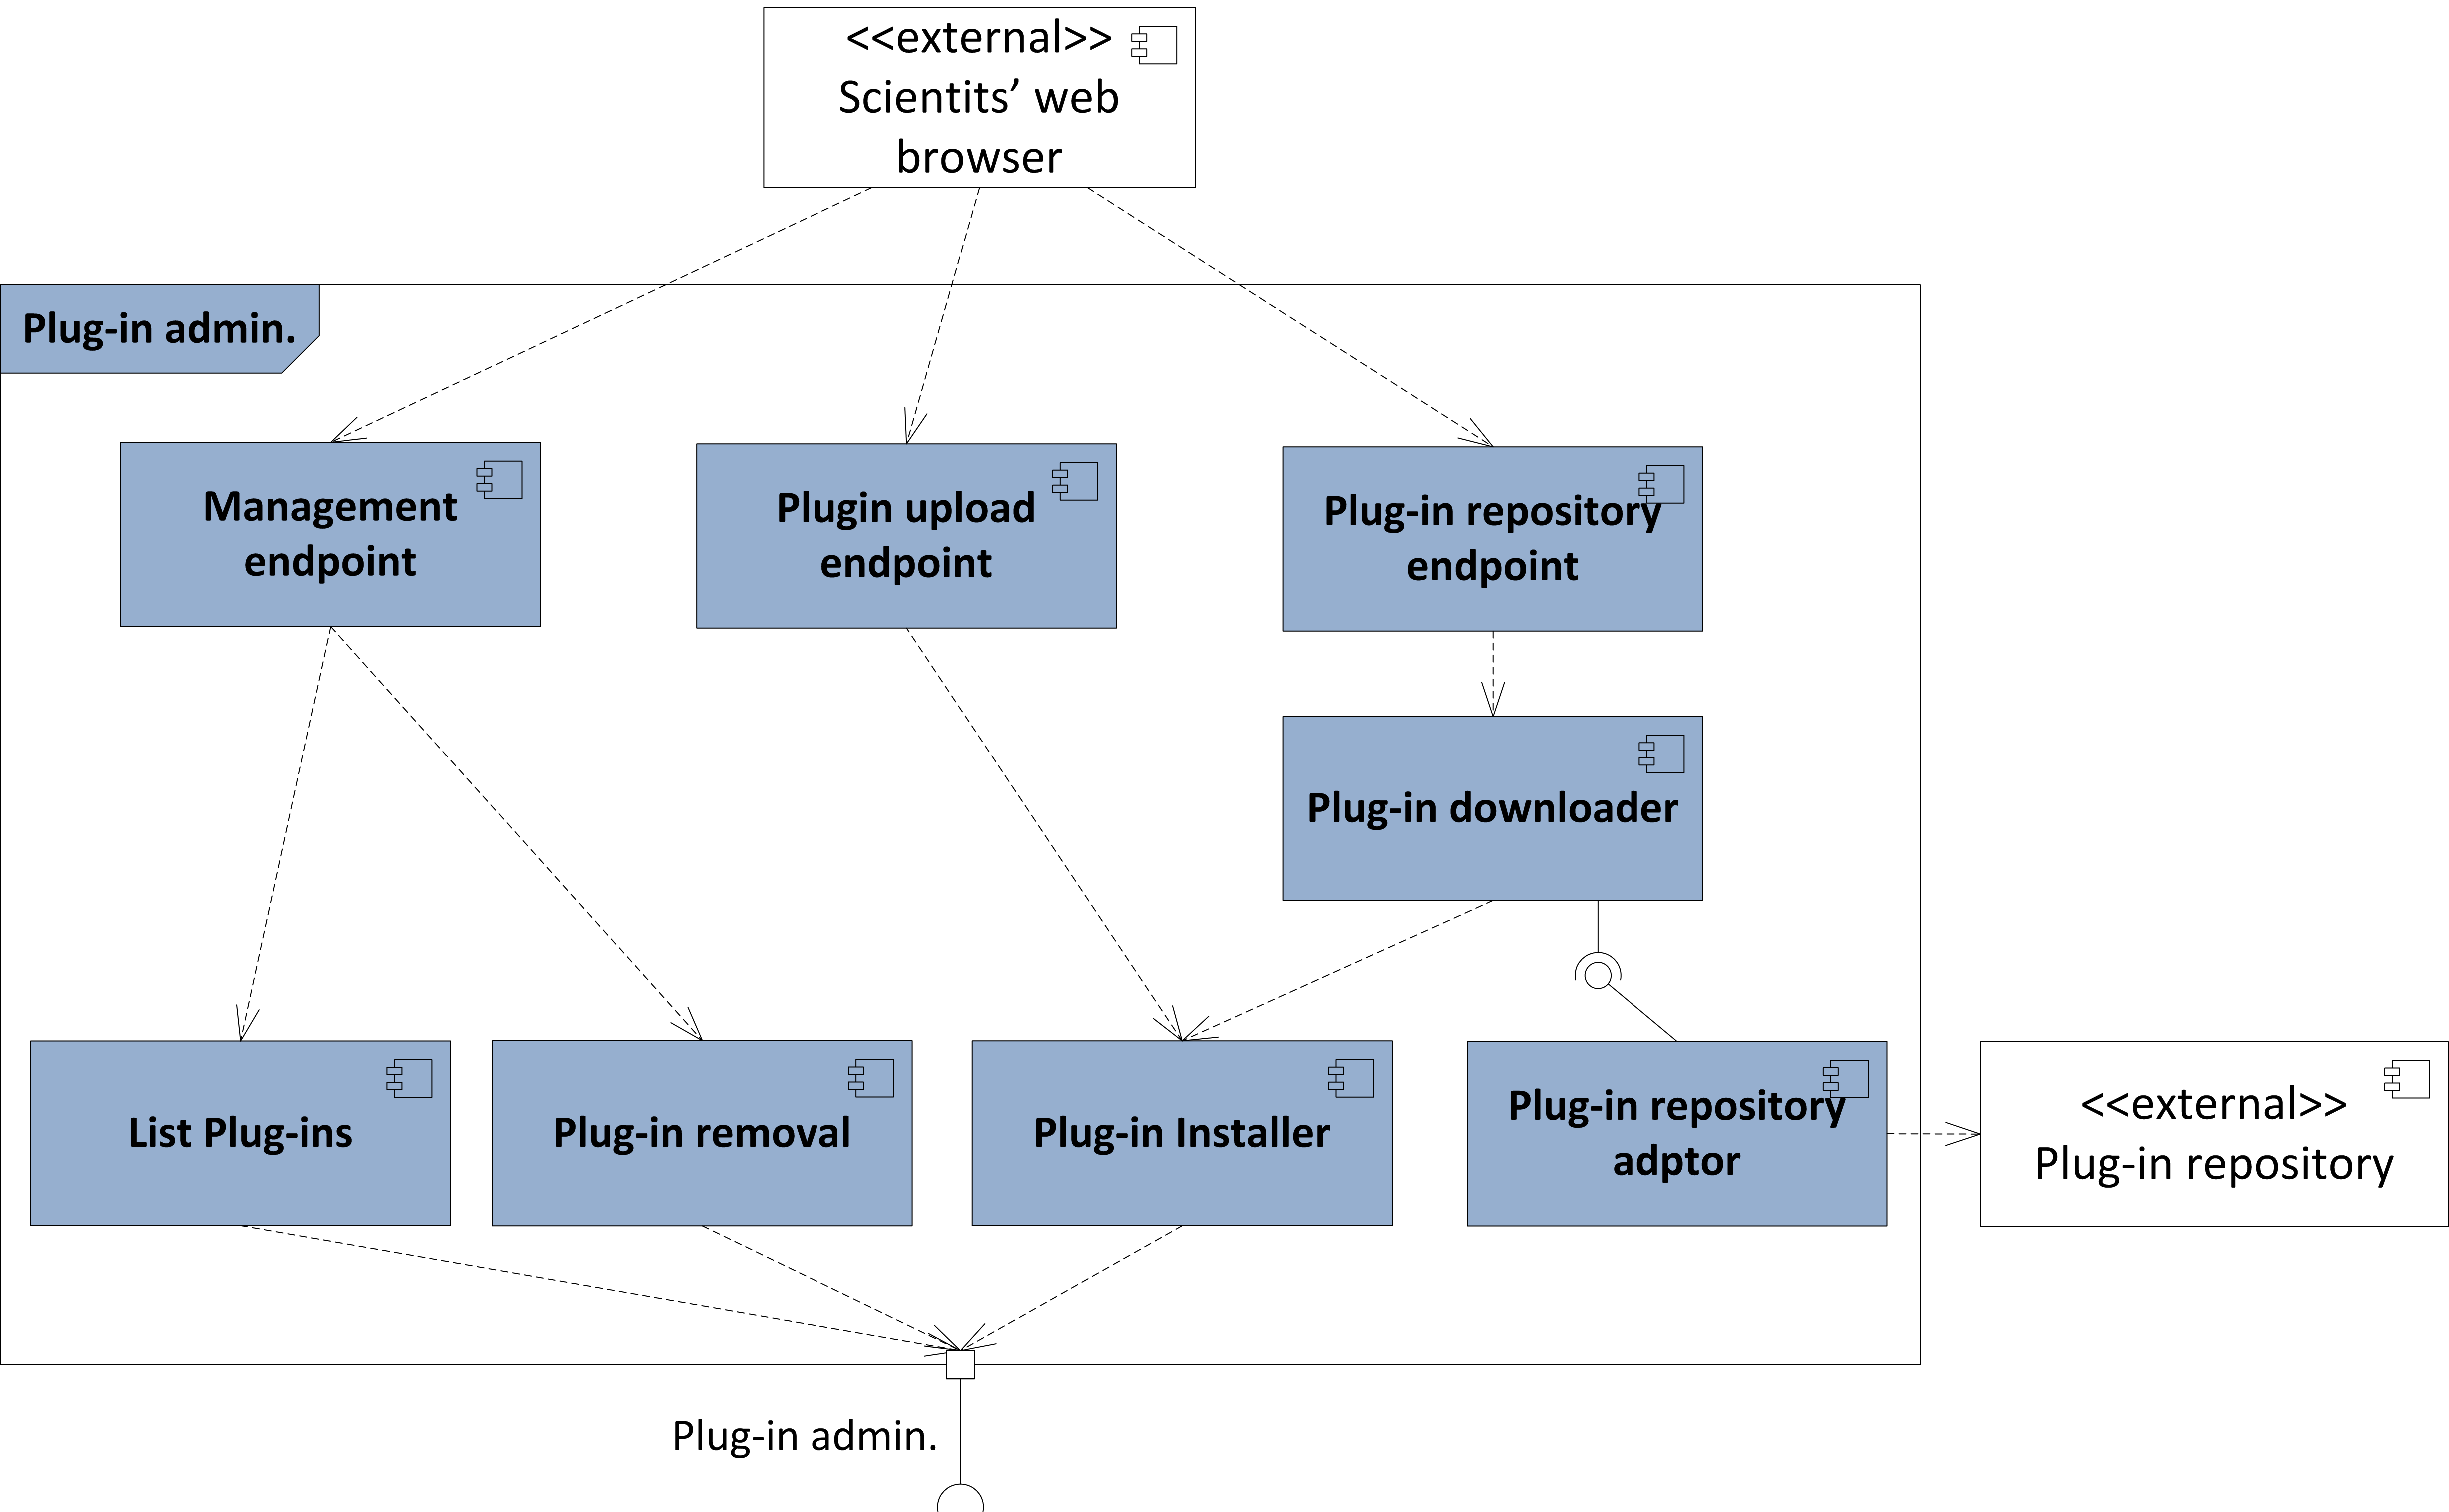
\includegraphics[scale=0.75]{plug-in/layers/admin-func.png}
  \caption{Layer organization of U-Sem}
\end{figure}

\begin{itemize}

\item \textit{List Plug-ins} - 

\item \textit{Plug-in removal} - 

\item \textit{Management endpoint} - 

\item \textit{Plug-in installer} - 

\item \textit{Plug-in upload endpoint} - 

\item \textit{Plug-in repository adaptor} - 

\item \textit{Plug-in downloader} - 

\item \textit{Plug-in repository endpoint} - 

\end{itemize}


\subsubsection{Plug-in access manager}

This component is responsible to provide endpoint for the administrators to manage the plug-ins. They can install and delete plug-ins. This component is responsible to store and manage the access to all plug-ins. \textbf{Figure} shows the functional decomposition of the Plug-in access manager module. It consists of the following components:


\begin{figure}[h!]
  \centering
  	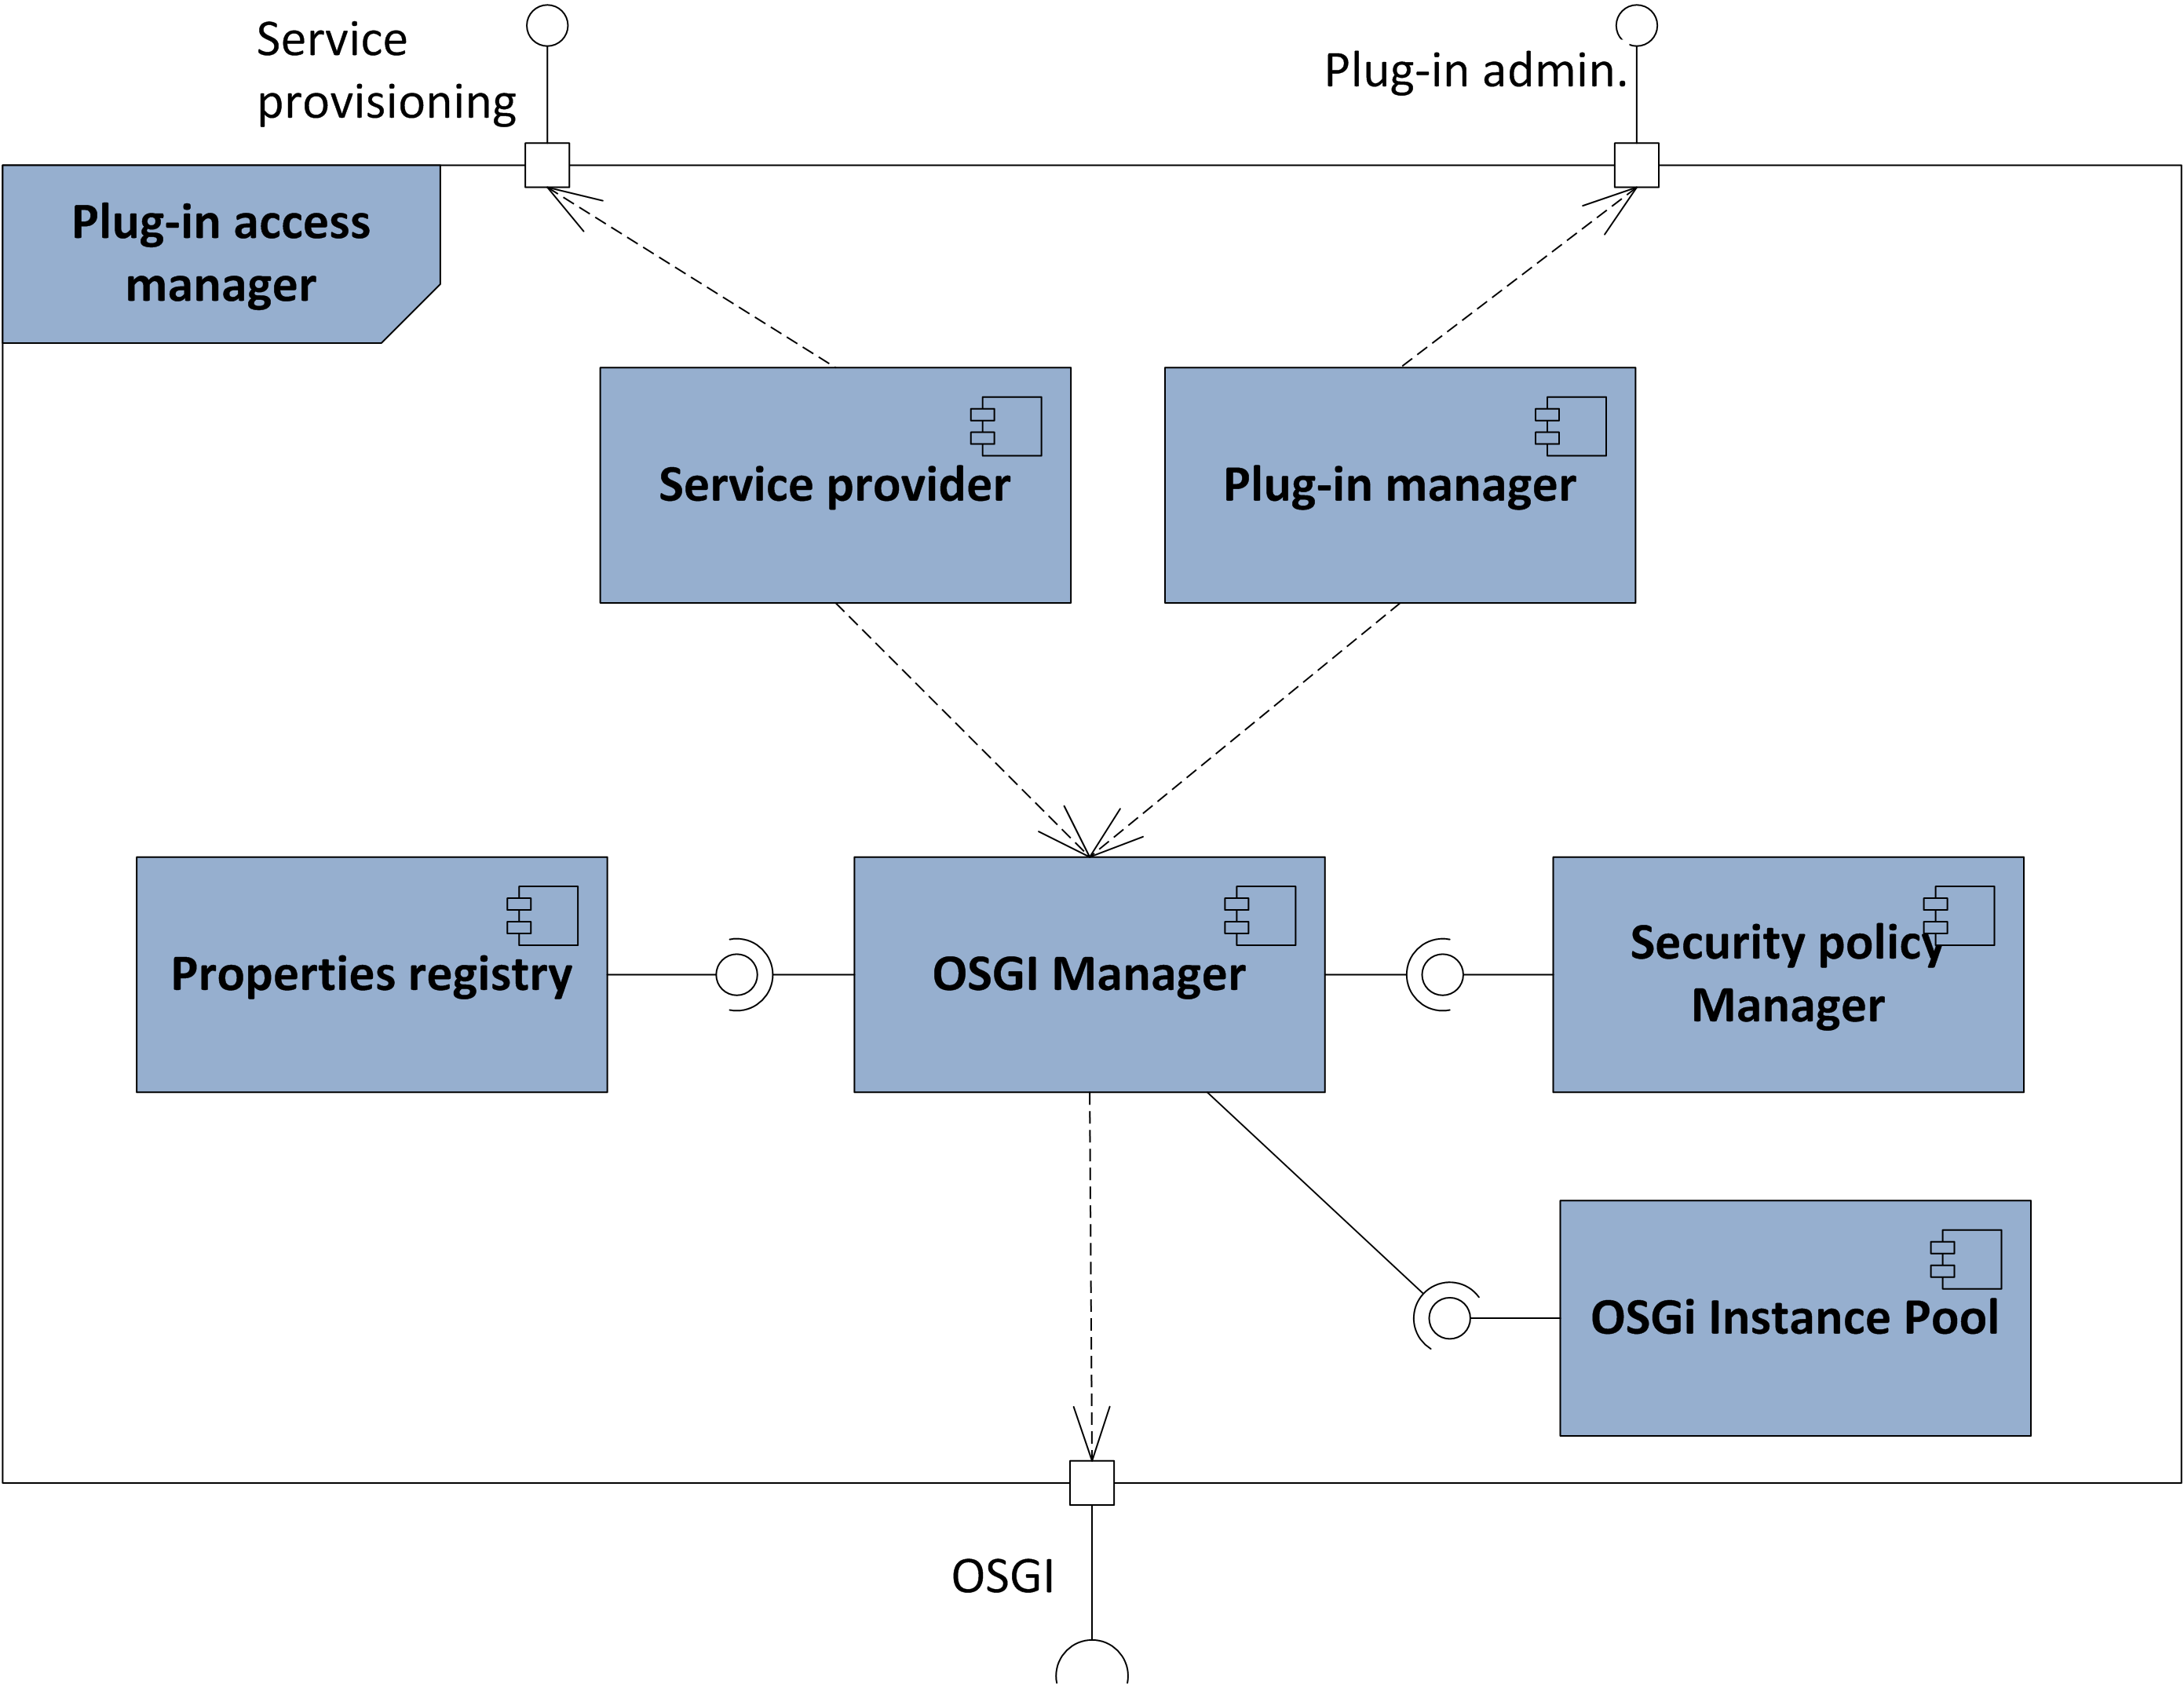
\includegraphics[scale=0.85]{plug-in/layers/access-func.png}
  \caption{Layer organization of U-Sem}
\end{figure}

\begin{itemize}

\item \textit{OSGI Adaptor} - 

\item \textit{Private space registry} - 

\item \textit{Security policy} - 

\item \textit{Plug-in manager} - 

\item \textit{Service provider} - 

\end{itemize}

\paragraph{Security}

\subsection{Concurent organization}

This section describes the concurrency structure of U-Sem. We show how functional elements map to concurrency units in order to clearly identify the parts of the system that can execute. We also show how this parallel execution is coordinated and controlled.

\begin{figure}[h!]
  \centering
  	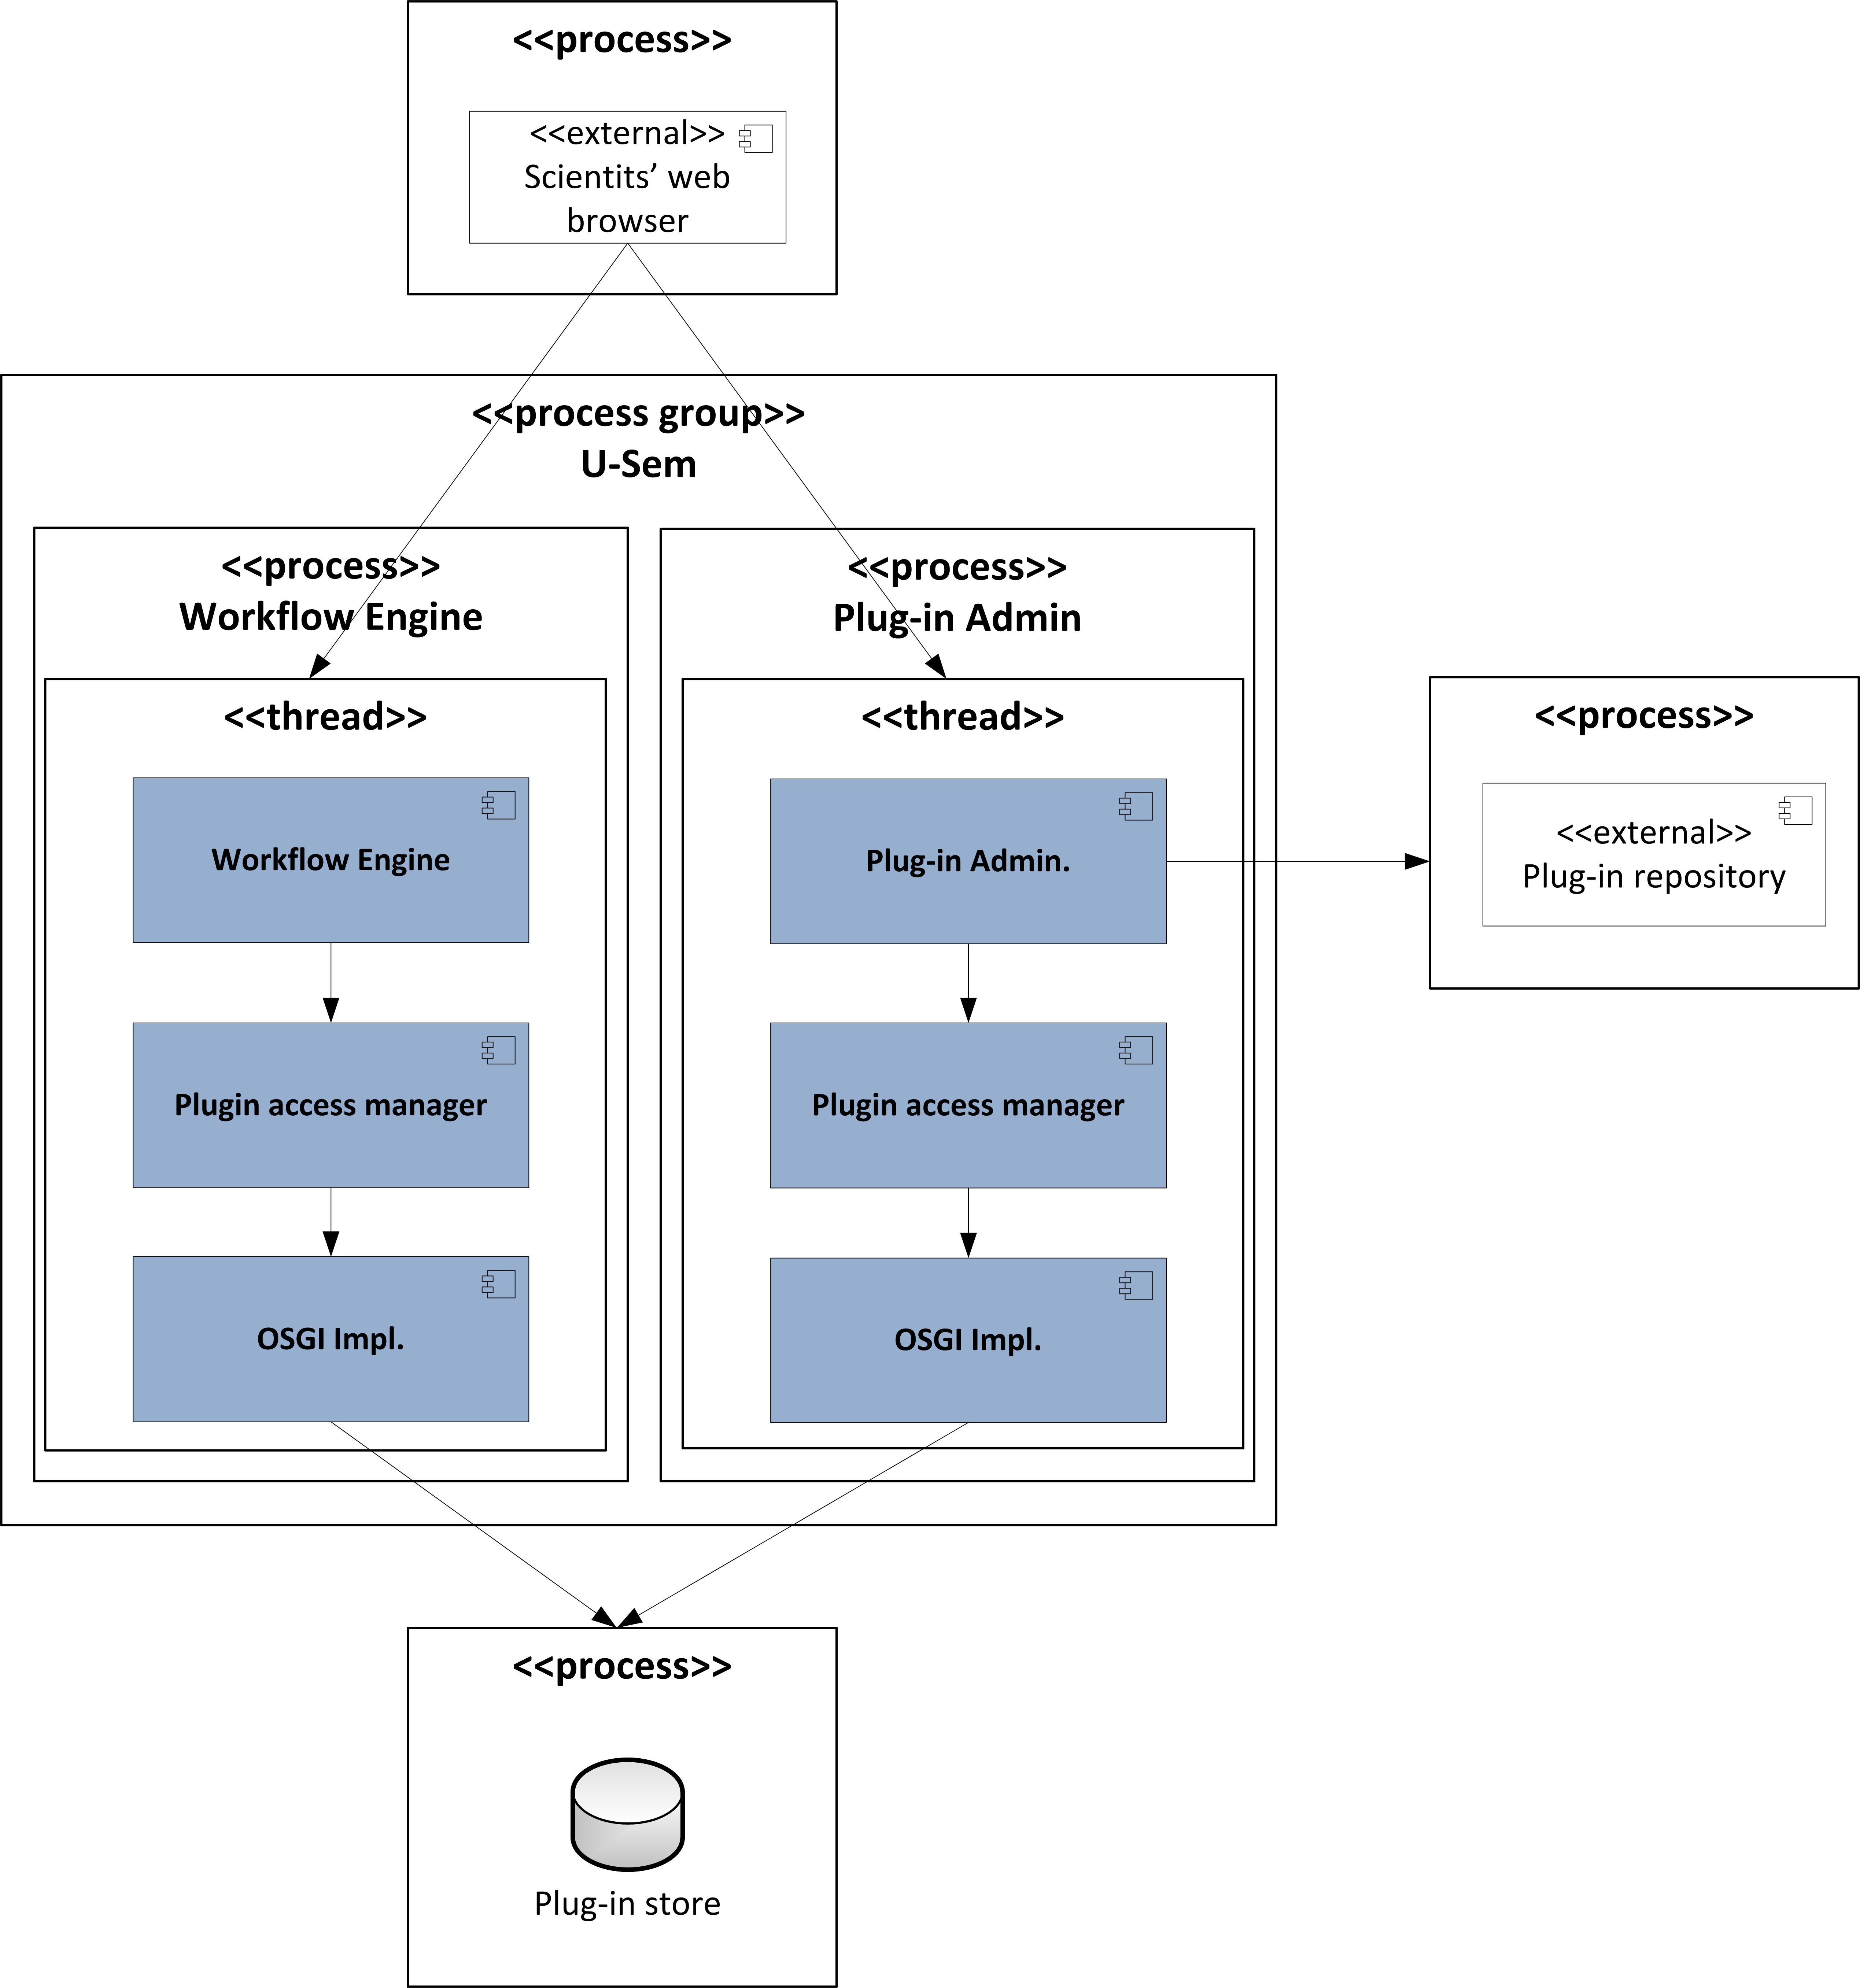
\includegraphics[scale=0.70]{plug-in/layers/concur.png}
  \caption{Layer organization of U-Sem}
\end{figure}

\section{Implementation}

In order to prove the applicabilities and capabilities of the system we actually implemented it.
osgi providers....

The component interfaces of U-Sem provide extension point where custom functionality provided by a component can be plugged in. Each component interface is represented by a java interface which defines the contract. \textbf{picture of socket}

The list of interfaces that U-Sem provides includes: functions and function descriptors, workflow templates, authentication modules......

local repository implementation

user interface

\section{Validation}

After successfully implementing the system we wanted to validate that the system complies with all functional and non-functional requirements discussed at the beginning of this chapter. In order to do this we performed an experiment. We tried to extract outside as a plug-in a functionality that is currently hardcoded into the workflow engine outside.

\subsection{Functional requirements}

\subsection{Non-functional requirements}



\section{Limitations and Future Work}

Most of the limitations and shortcomings of our approach are inherited from OSGI. 

\begin{thebibliography}{99}

\bibitem{Pour} G. Pour, Component-Based Software Development Approach: New Opportunities and Challenges, Proceedings Technology of Object-Oriented Languages, 1998. TOOLS 26., pp. 375-383.

\bibitem{Pour1}  G. Pour,  Enterprise JavaBeans,  JavaBeans and XML Expanding the Possibilities for Web-Based Enterprise Application Development,  Proceedings Technology of Object-Oriented Languages and Systems, 1999, TOOLS 31, pp.282-291.

\bibitem{Pour2} G.Pour, M. Griss, J. Favaro, Making the Transition to Component-Based Enterprise Software Development: Overcoming the Obstacles - Patterns for Success, Proceedings of Technology of Object-Oriented Languages and systems, 1999, pp.419 - 419.

\bibitem{Parnas} D. L. Parnas. On the criteria to be used in decomposing systems into modules. Communications of the ACM, 15(12):1053-1058, 1972.

\bibitem{Jifeng} H Jifeng, X Li, Z Liu, Component-based software engineering, Theoretical Aspects of Computing-ICTAC 2005

\bibitem{Cai} Cai, X. and Lyu, M.R. and Wong, K.F. and Ko, R, Component-based software engineering: technologies, development frameworks, and quality assurance schemes

\bibitem{Chen} Z Chen, Z Liu et al, Refinement and Verification in Component-Based Model Driven Design, Report of International Institute for Software Technology, 2007

\bibitem{Lau} Kung-Kiu Lau and Zheng Wang, Software Component Models

\bibitem{Bruneton} E. Bruneton, T. Coupaye, and J. Stefani, The Fractal Component Model, ObjectWeb Consortium, Technical Report Specification V2, 2003

\bibitem{OSGI} OSGi Alliance. http://www.osgi.org 

\bibitem{Andre} Andre L. C. Tavares, Marco Tulio Valente, A Gentle Introduction to OSGi

\bibitem{BPMN} Business Process Modeling Notation (BPMN) Specification, Final Adopted Specification. Technical report, Object Management Group (OMG), February 2006.

\bibitem{Decker} Decker, G. and Barros, A., Interaction modeling using BPMN, Business Process Management Workshops, 2008


\end{thebibliography}